\chapter{Implementation}
\label{chap:implementation}
The major contribution of our work is to provide a method in which 
convolutional neural networks can be trained to learn and play the game of 
chess. In this chapter, we will describe our dataset-- acquisition and its 
representation in sections~\ref{section:dataaq} and \ref{section:datarep} 
respectively. Then we discuss the details of the architectures we use 
(section~\ref{section:network-arch}), before moving on the algorithms to decide 
which move to play at the current board position 
(section~\ref{section:playing}).


\section{Training and Testing Dataset}
\label{section:dataaq}
We acquired two datasets from FICS Games 
Database\footnote{\url{http://www.ficsgames.org/}} website. The first 
one is a set of games played between chess players with average ELO rating 
greater than 2000 in the year 2014. The second one consists of 
the set of games played between computer chess engines played between 2009 and 
2014.


The set of games in each of the two datasets was fragmented into moves, where 
each move was represented by a board representation (described in the next 
section) and a label (the position of the piece moved and the position to which 
the piece was moved). We flip the board across the horizontal after flipping 
the color of each piece to convert the move made by the players with black 
pieces to the corresponding move by a player with white pieces. We discard the 
moves played by players with ELO rating less than 2000 since we had enough data 
to not consider them as an ``expert''. \\
%Is this a problem? Because white player always moves first. So we have the 
% black moves when an odd number of moves have taken place. Don't know if it 
% matters!
% The number of moves after augmenting the player 2 moves and discarding less 
% than 2000 ELO rating players' moves was 10M and 40M respectively.
We shuffle the data because of two reasons:
\begin{itemize} 
\item Our models and training procedures do not utilize the order in which the 
game was played. Each move is learnt with respect to the position of the pieces 
on the board.
\item We use batched stochastic gradient descent to learn the parameters of our 
models. Learning from consecutive samples can introduce high variance in the 
updates. This happens due to the strong correlations between consecutive 
samples 
and resultantly makes the learning procedure inefficient \cite{deepmind_nips}\\
The data-set was split as follows.
\end{itemize}

\begin{table}[H]
\centering
\begin{tabular}{@{}lll@{}}
\toprule
Dataset Name & Number of Games 	& Total number of boards  \\
\midrule
CvC 2009-14  & $370,480$	& $74,162,875$             \\ 
FICS 2014 (avg ELO$>$2000)    & $522,356$    	& $32,598,059$      \\
FICS 2014 (all ELO, subset) & $\sim 1M$ & $\sim 125M$\\
\bottomrule
\end{tabular}
\caption{Dataset sizes}
\end{table}

\begin{figure}
  \hspace{0.5in}
  \scalebox{.7}{%% Creator: Matplotlib, PGF backend
%%
%% To include the figure in your LaTeX document, write
%%   \input{<filename>.pgf}
%%
%% Make sure the required packages are loaded in your preamble
%%   \usepackage{pgf}
%%
%% Figures using additional raster images can only be included by \input if
%% they are in the same directory as the main LaTeX file. For loading figures
%% from other directories you can use the `import` package
%%   \usepackage{import}
%% and then include the figures with
%%   \import{<path to file>}{<filename>.pgf}
%%
%% Matplotlib used the following preamble
%%   \usepackage{fontspec}
%%   \setmainfont{DejaVu Serif}
%%   \setsansfont{DejaVu Sans}
%%   \setmonofont{DejaVu Sans Mono}
%%
\begingroup%
\makeatletter%
\begin{pgfpicture}%
\pgfpathrectangle{\pgfpointorigin}{\pgfqpoint{8.000000in}{6.000000in}}%
\pgfusepath{use as bounding box, clip}%
\begin{pgfscope}%
\pgfsetbuttcap%
\pgfsetmiterjoin%
\definecolor{currentfill}{rgb}{1.000000,1.000000,1.000000}%
\pgfsetfillcolor{currentfill}%
\pgfsetlinewidth{0.000000pt}%
\definecolor{currentstroke}{rgb}{1.000000,1.000000,1.000000}%
\pgfsetstrokecolor{currentstroke}%
\pgfsetdash{}{0pt}%
\pgfpathmoveto{\pgfqpoint{0.000000in}{0.000000in}}%
\pgfpathlineto{\pgfqpoint{8.000000in}{0.000000in}}%
\pgfpathlineto{\pgfqpoint{8.000000in}{6.000000in}}%
\pgfpathlineto{\pgfqpoint{0.000000in}{6.000000in}}%
\pgfpathclose%
\pgfusepath{fill}%
\end{pgfscope}%
\begin{pgfscope}%
\pgfsetbuttcap%
\pgfsetmiterjoin%
\definecolor{currentfill}{rgb}{1.000000,1.000000,1.000000}%
\pgfsetfillcolor{currentfill}%
\pgfsetlinewidth{0.000000pt}%
\definecolor{currentstroke}{rgb}{0.000000,0.000000,0.000000}%
\pgfsetstrokecolor{currentstroke}%
\pgfsetstrokeopacity{0.000000}%
\pgfsetdash{}{0pt}%
\pgfpathmoveto{\pgfqpoint{1.000000in}{0.600000in}}%
\pgfpathlineto{\pgfqpoint{7.200000in}{0.600000in}}%
\pgfpathlineto{\pgfqpoint{7.200000in}{5.400000in}}%
\pgfpathlineto{\pgfqpoint{1.000000in}{5.400000in}}%
\pgfpathclose%
\pgfusepath{fill}%
\end{pgfscope}%
\begin{pgfscope}%
\pgfpathrectangle{\pgfqpoint{1.000000in}{0.600000in}}{\pgfqpoint{6.200000in}{4.800000in}} %
\pgfusepath{clip}%
\pgfsetbuttcap%
\pgfsetmiterjoin%
\definecolor{currentfill}{rgb}{0.827451,0.827451,0.827451}%
\pgfsetfillcolor{currentfill}%
\pgfsetlinewidth{1.003750pt}%
\definecolor{currentstroke}{rgb}{0.000000,0.000000,0.000000}%
\pgfsetstrokecolor{currentstroke}%
\pgfsetdash{}{0pt}%
\pgfpathmoveto{\pgfqpoint{1.000000in}{0.600000in}}%
\pgfpathlineto{\pgfqpoint{1.258333in}{0.600000in}}%
\pgfpathlineto{\pgfqpoint{1.258333in}{5.180894in}}%
\pgfpathlineto{\pgfqpoint{1.000000in}{5.180894in}}%
\pgfpathlineto{\pgfqpoint{1.000000in}{0.600000in}}%
\pgfusepath{stroke,fill}%
\end{pgfscope}%
\begin{pgfscope}%
\pgfpathrectangle{\pgfqpoint{1.000000in}{0.600000in}}{\pgfqpoint{6.200000in}{4.800000in}} %
\pgfusepath{clip}%
\pgfsetbuttcap%
\pgfsetmiterjoin%
\definecolor{currentfill}{rgb}{0.827451,0.827451,0.827451}%
\pgfsetfillcolor{currentfill}%
\pgfsetlinewidth{1.003750pt}%
\definecolor{currentstroke}{rgb}{0.000000,0.000000,0.000000}%
\pgfsetstrokecolor{currentstroke}%
\pgfsetdash{}{0pt}%
\pgfpathmoveto{\pgfqpoint{2.033333in}{0.600000in}}%
\pgfpathlineto{\pgfqpoint{2.291667in}{0.600000in}}%
\pgfpathlineto{\pgfqpoint{2.291667in}{3.479202in}}%
\pgfpathlineto{\pgfqpoint{2.033333in}{3.479202in}}%
\pgfpathlineto{\pgfqpoint{2.033333in}{0.600000in}}%
\pgfusepath{stroke,fill}%
\end{pgfscope}%
\begin{pgfscope}%
\pgfpathrectangle{\pgfqpoint{1.000000in}{0.600000in}}{\pgfqpoint{6.200000in}{4.800000in}} %
\pgfusepath{clip}%
\pgfsetbuttcap%
\pgfsetmiterjoin%
\definecolor{currentfill}{rgb}{0.827451,0.827451,0.827451}%
\pgfsetfillcolor{currentfill}%
\pgfsetlinewidth{1.003750pt}%
\definecolor{currentstroke}{rgb}{0.000000,0.000000,0.000000}%
\pgfsetstrokecolor{currentstroke}%
\pgfsetdash{}{0pt}%
\pgfpathmoveto{\pgfqpoint{3.066667in}{0.600000in}}%
\pgfpathlineto{\pgfqpoint{3.325000in}{0.600000in}}%
\pgfpathlineto{\pgfqpoint{3.325000in}{3.442842in}}%
\pgfpathlineto{\pgfqpoint{3.066667in}{3.442842in}}%
\pgfpathlineto{\pgfqpoint{3.066667in}{0.600000in}}%
\pgfusepath{stroke,fill}%
\end{pgfscope}%
\begin{pgfscope}%
\pgfpathrectangle{\pgfqpoint{1.000000in}{0.600000in}}{\pgfqpoint{6.200000in}{4.800000in}} %
\pgfusepath{clip}%
\pgfsetbuttcap%
\pgfsetmiterjoin%
\definecolor{currentfill}{rgb}{0.827451,0.827451,0.827451}%
\pgfsetfillcolor{currentfill}%
\pgfsetlinewidth{1.003750pt}%
\definecolor{currentstroke}{rgb}{0.000000,0.000000,0.000000}%
\pgfsetstrokecolor{currentstroke}%
\pgfsetdash{}{0pt}%
\pgfpathmoveto{\pgfqpoint{4.100000in}{0.600000in}}%
\pgfpathlineto{\pgfqpoint{4.358333in}{0.600000in}}%
\pgfpathlineto{\pgfqpoint{4.358333in}{3.232154in}}%
\pgfpathlineto{\pgfqpoint{4.100000in}{3.232154in}}%
\pgfpathlineto{\pgfqpoint{4.100000in}{0.600000in}}%
\pgfusepath{stroke,fill}%
\end{pgfscope}%
\begin{pgfscope}%
\pgfpathrectangle{\pgfqpoint{1.000000in}{0.600000in}}{\pgfqpoint{6.200000in}{4.800000in}} %
\pgfusepath{clip}%
\pgfsetbuttcap%
\pgfsetmiterjoin%
\definecolor{currentfill}{rgb}{0.827451,0.827451,0.827451}%
\pgfsetfillcolor{currentfill}%
\pgfsetlinewidth{1.003750pt}%
\definecolor{currentstroke}{rgb}{0.000000,0.000000,0.000000}%
\pgfsetstrokecolor{currentstroke}%
\pgfsetdash{}{0pt}%
\pgfpathmoveto{\pgfqpoint{5.133333in}{0.600000in}}%
\pgfpathlineto{\pgfqpoint{5.391667in}{0.600000in}}%
\pgfpathlineto{\pgfqpoint{5.391667in}{2.688066in}}%
\pgfpathlineto{\pgfqpoint{5.133333in}{2.688066in}}%
\pgfpathlineto{\pgfqpoint{5.133333in}{0.600000in}}%
\pgfusepath{stroke,fill}%
\end{pgfscope}%
\begin{pgfscope}%
\pgfpathrectangle{\pgfqpoint{1.000000in}{0.600000in}}{\pgfqpoint{6.200000in}{4.800000in}} %
\pgfusepath{clip}%
\pgfsetbuttcap%
\pgfsetmiterjoin%
\definecolor{currentfill}{rgb}{0.827451,0.827451,0.827451}%
\pgfsetfillcolor{currentfill}%
\pgfsetlinewidth{1.003750pt}%
\definecolor{currentstroke}{rgb}{0.000000,0.000000,0.000000}%
\pgfsetstrokecolor{currentstroke}%
\pgfsetdash{}{0pt}%
\pgfpathmoveto{\pgfqpoint{6.166667in}{0.600000in}}%
\pgfpathlineto{\pgfqpoint{6.425000in}{0.600000in}}%
\pgfpathlineto{\pgfqpoint{6.425000in}{2.962474in}}%
\pgfpathlineto{\pgfqpoint{6.166667in}{2.962474in}}%
\pgfpathlineto{\pgfqpoint{6.166667in}{0.600000in}}%
\pgfusepath{stroke,fill}%
\end{pgfscope}%
\begin{pgfscope}%
\pgfpathrectangle{\pgfqpoint{1.000000in}{0.600000in}}{\pgfqpoint{6.200000in}{4.800000in}} %
\pgfusepath{clip}%
\pgfsetbuttcap%
\pgfsetmiterjoin%
\definecolor{currentfill}{rgb}{0.117647,0.564706,1.000000}%
\pgfsetfillcolor{currentfill}%
\pgfsetlinewidth{1.003750pt}%
\definecolor{currentstroke}{rgb}{0.000000,0.000000,0.000000}%
\pgfsetstrokecolor{currentstroke}%
\pgfsetdash{}{0pt}%
\pgfpathmoveto{\pgfqpoint{1.258333in}{0.600000in}}%
\pgfpathlineto{\pgfqpoint{1.516667in}{0.600000in}}%
\pgfpathlineto{\pgfqpoint{1.516667in}{5.381416in}}%
\pgfpathlineto{\pgfqpoint{1.258333in}{5.381416in}}%
\pgfpathlineto{\pgfqpoint{1.258333in}{0.600000in}}%
\pgfusepath{stroke,fill}%
\end{pgfscope}%
\begin{pgfscope}%
\pgfpathrectangle{\pgfqpoint{1.000000in}{0.600000in}}{\pgfqpoint{6.200000in}{4.800000in}} %
\pgfusepath{clip}%
\pgfsetbuttcap%
\pgfsetmiterjoin%
\definecolor{currentfill}{rgb}{0.117647,0.564706,1.000000}%
\pgfsetfillcolor{currentfill}%
\pgfsetlinewidth{1.003750pt}%
\definecolor{currentstroke}{rgb}{0.000000,0.000000,0.000000}%
\pgfsetstrokecolor{currentstroke}%
\pgfsetdash{}{0pt}%
\pgfpathmoveto{\pgfqpoint{2.291667in}{0.600000in}}%
\pgfpathlineto{\pgfqpoint{2.550000in}{0.600000in}}%
\pgfpathlineto{\pgfqpoint{2.550000in}{5.009714in}}%
\pgfpathlineto{\pgfqpoint{2.291667in}{5.009714in}}%
\pgfpathlineto{\pgfqpoint{2.291667in}{0.600000in}}%
\pgfusepath{stroke,fill}%
\end{pgfscope}%
\begin{pgfscope}%
\pgfpathrectangle{\pgfqpoint{1.000000in}{0.600000in}}{\pgfqpoint{6.200000in}{4.800000in}} %
\pgfusepath{clip}%
\pgfsetbuttcap%
\pgfsetmiterjoin%
\definecolor{currentfill}{rgb}{0.117647,0.564706,1.000000}%
\pgfsetfillcolor{currentfill}%
\pgfsetlinewidth{1.003750pt}%
\definecolor{currentstroke}{rgb}{0.000000,0.000000,0.000000}%
\pgfsetstrokecolor{currentstroke}%
\pgfsetdash{}{0pt}%
\pgfpathmoveto{\pgfqpoint{3.325000in}{0.600000in}}%
\pgfpathlineto{\pgfqpoint{3.583333in}{0.600000in}}%
\pgfpathlineto{\pgfqpoint{3.583333in}{3.555010in}}%
\pgfpathlineto{\pgfqpoint{3.325000in}{3.555010in}}%
\pgfpathlineto{\pgfqpoint{3.325000in}{0.600000in}}%
\pgfusepath{stroke,fill}%
\end{pgfscope}%
\begin{pgfscope}%
\pgfpathrectangle{\pgfqpoint{1.000000in}{0.600000in}}{\pgfqpoint{6.200000in}{4.800000in}} %
\pgfusepath{clip}%
\pgfsetbuttcap%
\pgfsetmiterjoin%
\definecolor{currentfill}{rgb}{0.117647,0.564706,1.000000}%
\pgfsetfillcolor{currentfill}%
\pgfsetlinewidth{1.003750pt}%
\definecolor{currentstroke}{rgb}{0.000000,0.000000,0.000000}%
\pgfsetstrokecolor{currentstroke}%
\pgfsetdash{}{0pt}%
\pgfpathmoveto{\pgfqpoint{4.358333in}{0.600000in}}%
\pgfpathlineto{\pgfqpoint{4.616667in}{0.600000in}}%
\pgfpathlineto{\pgfqpoint{4.616667in}{3.841903in}}%
\pgfpathlineto{\pgfqpoint{4.358333in}{3.841903in}}%
\pgfpathlineto{\pgfqpoint{4.358333in}{0.600000in}}%
\pgfusepath{stroke,fill}%
\end{pgfscope}%
\begin{pgfscope}%
\pgfpathrectangle{\pgfqpoint{1.000000in}{0.600000in}}{\pgfqpoint{6.200000in}{4.800000in}} %
\pgfusepath{clip}%
\pgfsetbuttcap%
\pgfsetmiterjoin%
\definecolor{currentfill}{rgb}{0.117647,0.564706,1.000000}%
\pgfsetfillcolor{currentfill}%
\pgfsetlinewidth{1.003750pt}%
\definecolor{currentstroke}{rgb}{0.000000,0.000000,0.000000}%
\pgfsetstrokecolor{currentstroke}%
\pgfsetdash{}{0pt}%
\pgfpathmoveto{\pgfqpoint{5.391667in}{0.600000in}}%
\pgfpathlineto{\pgfqpoint{5.650000in}{0.600000in}}%
\pgfpathlineto{\pgfqpoint{5.650000in}{3.505016in}}%
\pgfpathlineto{\pgfqpoint{5.391667in}{3.505016in}}%
\pgfpathlineto{\pgfqpoint{5.391667in}{0.600000in}}%
\pgfusepath{stroke,fill}%
\end{pgfscope}%
\begin{pgfscope}%
\pgfpathrectangle{\pgfqpoint{1.000000in}{0.600000in}}{\pgfqpoint{6.200000in}{4.800000in}} %
\pgfusepath{clip}%
\pgfsetbuttcap%
\pgfsetmiterjoin%
\definecolor{currentfill}{rgb}{0.117647,0.564706,1.000000}%
\pgfsetfillcolor{currentfill}%
\pgfsetlinewidth{1.003750pt}%
\definecolor{currentstroke}{rgb}{0.000000,0.000000,0.000000}%
\pgfsetstrokecolor{currentstroke}%
\pgfsetdash{}{0pt}%
\pgfpathmoveto{\pgfqpoint{6.425000in}{0.600000in}}%
\pgfpathlineto{\pgfqpoint{6.683333in}{0.600000in}}%
\pgfpathlineto{\pgfqpoint{6.683333in}{4.474843in}}%
\pgfpathlineto{\pgfqpoint{6.425000in}{4.474843in}}%
\pgfpathlineto{\pgfqpoint{6.425000in}{0.600000in}}%
\pgfusepath{stroke,fill}%
\end{pgfscope}%
\begin{pgfscope}%
\pgfsetrectcap%
\pgfsetmiterjoin%
\pgfsetlinewidth{1.003750pt}%
\definecolor{currentstroke}{rgb}{0.000000,0.000000,0.000000}%
\pgfsetstrokecolor{currentstroke}%
\pgfsetdash{}{0pt}%
\pgfpathmoveto{\pgfqpoint{1.000000in}{5.400000in}}%
\pgfpathlineto{\pgfqpoint{7.200000in}{5.400000in}}%
\pgfusepath{stroke}%
\end{pgfscope}%
\begin{pgfscope}%
\pgfsetrectcap%
\pgfsetmiterjoin%
\pgfsetlinewidth{1.003750pt}%
\definecolor{currentstroke}{rgb}{0.000000,0.000000,0.000000}%
\pgfsetstrokecolor{currentstroke}%
\pgfsetdash{}{0pt}%
\pgfpathmoveto{\pgfqpoint{7.200000in}{0.600000in}}%
\pgfpathlineto{\pgfqpoint{7.200000in}{5.400000in}}%
\pgfusepath{stroke}%
\end{pgfscope}%
\begin{pgfscope}%
\pgfsetrectcap%
\pgfsetmiterjoin%
\pgfsetlinewidth{1.003750pt}%
\definecolor{currentstroke}{rgb}{0.000000,0.000000,0.000000}%
\pgfsetstrokecolor{currentstroke}%
\pgfsetdash{}{0pt}%
\pgfpathmoveto{\pgfqpoint{1.000000in}{0.600000in}}%
\pgfpathlineto{\pgfqpoint{7.200000in}{0.600000in}}%
\pgfusepath{stroke}%
\end{pgfscope}%
\begin{pgfscope}%
\pgfsetrectcap%
\pgfsetmiterjoin%
\pgfsetlinewidth{1.003750pt}%
\definecolor{currentstroke}{rgb}{0.000000,0.000000,0.000000}%
\pgfsetstrokecolor{currentstroke}%
\pgfsetdash{}{0pt}%
\pgfpathmoveto{\pgfqpoint{1.000000in}{0.600000in}}%
\pgfpathlineto{\pgfqpoint{1.000000in}{5.400000in}}%
\pgfusepath{stroke}%
\end{pgfscope}%
\begin{pgfscope}%
\pgfsetbuttcap%
\pgfsetroundjoin%
\definecolor{currentfill}{rgb}{0.000000,0.000000,0.000000}%
\pgfsetfillcolor{currentfill}%
\pgfsetlinewidth{0.501875pt}%
\definecolor{currentstroke}{rgb}{0.000000,0.000000,0.000000}%
\pgfsetstrokecolor{currentstroke}%
\pgfsetdash{}{0pt}%
\pgfsys@defobject{currentmarker}{\pgfqpoint{0.000000in}{0.000000in}}{\pgfqpoint{0.000000in}{0.055556in}}{%
\pgfpathmoveto{\pgfqpoint{0.000000in}{0.000000in}}%
\pgfpathlineto{\pgfqpoint{0.000000in}{0.055556in}}%
\pgfusepath{stroke,fill}%
}%
\begin{pgfscope}%
\pgfsys@transformshift{1.258333in}{0.600000in}%
\pgfsys@useobject{currentmarker}{}%
\end{pgfscope}%
\end{pgfscope}%
\begin{pgfscope}%
\pgfsetbuttcap%
\pgfsetroundjoin%
\definecolor{currentfill}{rgb}{0.000000,0.000000,0.000000}%
\pgfsetfillcolor{currentfill}%
\pgfsetlinewidth{0.501875pt}%
\definecolor{currentstroke}{rgb}{0.000000,0.000000,0.000000}%
\pgfsetstrokecolor{currentstroke}%
\pgfsetdash{}{0pt}%
\pgfsys@defobject{currentmarker}{\pgfqpoint{0.000000in}{-0.055556in}}{\pgfqpoint{0.000000in}{0.000000in}}{%
\pgfpathmoveto{\pgfqpoint{0.000000in}{0.000000in}}%
\pgfpathlineto{\pgfqpoint{0.000000in}{-0.055556in}}%
\pgfusepath{stroke,fill}%
}%
\begin{pgfscope}%
\pgfsys@transformshift{1.258333in}{5.400000in}%
\pgfsys@useobject{currentmarker}{}%
\end{pgfscope}%
\end{pgfscope}%
\begin{pgfscope}%
\pgftext[x=1.258333in,y=0.544444in,,top]{\rmfamily\fontsize{12.000000}{14.400000}\selectfont Pawn}%
\end{pgfscope}%
\begin{pgfscope}%
\pgfsetbuttcap%
\pgfsetroundjoin%
\definecolor{currentfill}{rgb}{0.000000,0.000000,0.000000}%
\pgfsetfillcolor{currentfill}%
\pgfsetlinewidth{0.501875pt}%
\definecolor{currentstroke}{rgb}{0.000000,0.000000,0.000000}%
\pgfsetstrokecolor{currentstroke}%
\pgfsetdash{}{0pt}%
\pgfsys@defobject{currentmarker}{\pgfqpoint{0.000000in}{0.000000in}}{\pgfqpoint{0.000000in}{0.055556in}}{%
\pgfpathmoveto{\pgfqpoint{0.000000in}{0.000000in}}%
\pgfpathlineto{\pgfqpoint{0.000000in}{0.055556in}}%
\pgfusepath{stroke,fill}%
}%
\begin{pgfscope}%
\pgfsys@transformshift{2.291667in}{0.600000in}%
\pgfsys@useobject{currentmarker}{}%
\end{pgfscope}%
\end{pgfscope}%
\begin{pgfscope}%
\pgfsetbuttcap%
\pgfsetroundjoin%
\definecolor{currentfill}{rgb}{0.000000,0.000000,0.000000}%
\pgfsetfillcolor{currentfill}%
\pgfsetlinewidth{0.501875pt}%
\definecolor{currentstroke}{rgb}{0.000000,0.000000,0.000000}%
\pgfsetstrokecolor{currentstroke}%
\pgfsetdash{}{0pt}%
\pgfsys@defobject{currentmarker}{\pgfqpoint{0.000000in}{-0.055556in}}{\pgfqpoint{0.000000in}{0.000000in}}{%
\pgfpathmoveto{\pgfqpoint{0.000000in}{0.000000in}}%
\pgfpathlineto{\pgfqpoint{0.000000in}{-0.055556in}}%
\pgfusepath{stroke,fill}%
}%
\begin{pgfscope}%
\pgfsys@transformshift{2.291667in}{5.400000in}%
\pgfsys@useobject{currentmarker}{}%
\end{pgfscope}%
\end{pgfscope}%
\begin{pgfscope}%
\pgftext[x=2.291667in,y=0.544444in,,top]{\rmfamily\fontsize{12.000000}{14.400000}\selectfont Rook}%
\end{pgfscope}%
\begin{pgfscope}%
\pgfsetbuttcap%
\pgfsetroundjoin%
\definecolor{currentfill}{rgb}{0.000000,0.000000,0.000000}%
\pgfsetfillcolor{currentfill}%
\pgfsetlinewidth{0.501875pt}%
\definecolor{currentstroke}{rgb}{0.000000,0.000000,0.000000}%
\pgfsetstrokecolor{currentstroke}%
\pgfsetdash{}{0pt}%
\pgfsys@defobject{currentmarker}{\pgfqpoint{0.000000in}{0.000000in}}{\pgfqpoint{0.000000in}{0.055556in}}{%
\pgfpathmoveto{\pgfqpoint{0.000000in}{0.000000in}}%
\pgfpathlineto{\pgfqpoint{0.000000in}{0.055556in}}%
\pgfusepath{stroke,fill}%
}%
\begin{pgfscope}%
\pgfsys@transformshift{3.325000in}{0.600000in}%
\pgfsys@useobject{currentmarker}{}%
\end{pgfscope}%
\end{pgfscope}%
\begin{pgfscope}%
\pgfsetbuttcap%
\pgfsetroundjoin%
\definecolor{currentfill}{rgb}{0.000000,0.000000,0.000000}%
\pgfsetfillcolor{currentfill}%
\pgfsetlinewidth{0.501875pt}%
\definecolor{currentstroke}{rgb}{0.000000,0.000000,0.000000}%
\pgfsetstrokecolor{currentstroke}%
\pgfsetdash{}{0pt}%
\pgfsys@defobject{currentmarker}{\pgfqpoint{0.000000in}{-0.055556in}}{\pgfqpoint{0.000000in}{0.000000in}}{%
\pgfpathmoveto{\pgfqpoint{0.000000in}{0.000000in}}%
\pgfpathlineto{\pgfqpoint{0.000000in}{-0.055556in}}%
\pgfusepath{stroke,fill}%
}%
\begin{pgfscope}%
\pgfsys@transformshift{3.325000in}{5.400000in}%
\pgfsys@useobject{currentmarker}{}%
\end{pgfscope}%
\end{pgfscope}%
\begin{pgfscope}%
\pgftext[x=3.325000in,y=0.544444in,,top]{\rmfamily\fontsize{12.000000}{14.400000}\selectfont Knight}%
\end{pgfscope}%
\begin{pgfscope}%
\pgfsetbuttcap%
\pgfsetroundjoin%
\definecolor{currentfill}{rgb}{0.000000,0.000000,0.000000}%
\pgfsetfillcolor{currentfill}%
\pgfsetlinewidth{0.501875pt}%
\definecolor{currentstroke}{rgb}{0.000000,0.000000,0.000000}%
\pgfsetstrokecolor{currentstroke}%
\pgfsetdash{}{0pt}%
\pgfsys@defobject{currentmarker}{\pgfqpoint{0.000000in}{0.000000in}}{\pgfqpoint{0.000000in}{0.055556in}}{%
\pgfpathmoveto{\pgfqpoint{0.000000in}{0.000000in}}%
\pgfpathlineto{\pgfqpoint{0.000000in}{0.055556in}}%
\pgfusepath{stroke,fill}%
}%
\begin{pgfscope}%
\pgfsys@transformshift{4.358333in}{0.600000in}%
\pgfsys@useobject{currentmarker}{}%
\end{pgfscope}%
\end{pgfscope}%
\begin{pgfscope}%
\pgfsetbuttcap%
\pgfsetroundjoin%
\definecolor{currentfill}{rgb}{0.000000,0.000000,0.000000}%
\pgfsetfillcolor{currentfill}%
\pgfsetlinewidth{0.501875pt}%
\definecolor{currentstroke}{rgb}{0.000000,0.000000,0.000000}%
\pgfsetstrokecolor{currentstroke}%
\pgfsetdash{}{0pt}%
\pgfsys@defobject{currentmarker}{\pgfqpoint{0.000000in}{-0.055556in}}{\pgfqpoint{0.000000in}{0.000000in}}{%
\pgfpathmoveto{\pgfqpoint{0.000000in}{0.000000in}}%
\pgfpathlineto{\pgfqpoint{0.000000in}{-0.055556in}}%
\pgfusepath{stroke,fill}%
}%
\begin{pgfscope}%
\pgfsys@transformshift{4.358333in}{5.400000in}%
\pgfsys@useobject{currentmarker}{}%
\end{pgfscope}%
\end{pgfscope}%
\begin{pgfscope}%
\pgftext[x=4.358333in,y=0.544444in,,top]{\rmfamily\fontsize{12.000000}{14.400000}\selectfont Bishop}%
\end{pgfscope}%
\begin{pgfscope}%
\pgfsetbuttcap%
\pgfsetroundjoin%
\definecolor{currentfill}{rgb}{0.000000,0.000000,0.000000}%
\pgfsetfillcolor{currentfill}%
\pgfsetlinewidth{0.501875pt}%
\definecolor{currentstroke}{rgb}{0.000000,0.000000,0.000000}%
\pgfsetstrokecolor{currentstroke}%
\pgfsetdash{}{0pt}%
\pgfsys@defobject{currentmarker}{\pgfqpoint{0.000000in}{0.000000in}}{\pgfqpoint{0.000000in}{0.055556in}}{%
\pgfpathmoveto{\pgfqpoint{0.000000in}{0.000000in}}%
\pgfpathlineto{\pgfqpoint{0.000000in}{0.055556in}}%
\pgfusepath{stroke,fill}%
}%
\begin{pgfscope}%
\pgfsys@transformshift{5.391667in}{0.600000in}%
\pgfsys@useobject{currentmarker}{}%
\end{pgfscope}%
\end{pgfscope}%
\begin{pgfscope}%
\pgfsetbuttcap%
\pgfsetroundjoin%
\definecolor{currentfill}{rgb}{0.000000,0.000000,0.000000}%
\pgfsetfillcolor{currentfill}%
\pgfsetlinewidth{0.501875pt}%
\definecolor{currentstroke}{rgb}{0.000000,0.000000,0.000000}%
\pgfsetstrokecolor{currentstroke}%
\pgfsetdash{}{0pt}%
\pgfsys@defobject{currentmarker}{\pgfqpoint{0.000000in}{-0.055556in}}{\pgfqpoint{0.000000in}{0.000000in}}{%
\pgfpathmoveto{\pgfqpoint{0.000000in}{0.000000in}}%
\pgfpathlineto{\pgfqpoint{0.000000in}{-0.055556in}}%
\pgfusepath{stroke,fill}%
}%
\begin{pgfscope}%
\pgfsys@transformshift{5.391667in}{5.400000in}%
\pgfsys@useobject{currentmarker}{}%
\end{pgfscope}%
\end{pgfscope}%
\begin{pgfscope}%
\pgftext[x=5.391667in,y=0.544444in,,top]{\rmfamily\fontsize{12.000000}{14.400000}\selectfont Queen}%
\end{pgfscope}%
\begin{pgfscope}%
\pgfsetbuttcap%
\pgfsetroundjoin%
\definecolor{currentfill}{rgb}{0.000000,0.000000,0.000000}%
\pgfsetfillcolor{currentfill}%
\pgfsetlinewidth{0.501875pt}%
\definecolor{currentstroke}{rgb}{0.000000,0.000000,0.000000}%
\pgfsetstrokecolor{currentstroke}%
\pgfsetdash{}{0pt}%
\pgfsys@defobject{currentmarker}{\pgfqpoint{0.000000in}{0.000000in}}{\pgfqpoint{0.000000in}{0.055556in}}{%
\pgfpathmoveto{\pgfqpoint{0.000000in}{0.000000in}}%
\pgfpathlineto{\pgfqpoint{0.000000in}{0.055556in}}%
\pgfusepath{stroke,fill}%
}%
\begin{pgfscope}%
\pgfsys@transformshift{6.425000in}{0.600000in}%
\pgfsys@useobject{currentmarker}{}%
\end{pgfscope}%
\end{pgfscope}%
\begin{pgfscope}%
\pgfsetbuttcap%
\pgfsetroundjoin%
\definecolor{currentfill}{rgb}{0.000000,0.000000,0.000000}%
\pgfsetfillcolor{currentfill}%
\pgfsetlinewidth{0.501875pt}%
\definecolor{currentstroke}{rgb}{0.000000,0.000000,0.000000}%
\pgfsetstrokecolor{currentstroke}%
\pgfsetdash{}{0pt}%
\pgfsys@defobject{currentmarker}{\pgfqpoint{0.000000in}{-0.055556in}}{\pgfqpoint{0.000000in}{0.000000in}}{%
\pgfpathmoveto{\pgfqpoint{0.000000in}{0.000000in}}%
\pgfpathlineto{\pgfqpoint{0.000000in}{-0.055556in}}%
\pgfusepath{stroke,fill}%
}%
\begin{pgfscope}%
\pgfsys@transformshift{6.425000in}{5.400000in}%
\pgfsys@useobject{currentmarker}{}%
\end{pgfscope}%
\end{pgfscope}%
\begin{pgfscope}%
\pgftext[x=6.425000in,y=0.544444in,,top]{\rmfamily\fontsize{12.000000}{14.400000}\selectfont King}%
\end{pgfscope}%
\begin{pgfscope}%
\pgftext[x=4.100000in,y=0.311345in,,top]{\rmfamily\fontsize{12.000000}{14.400000}\selectfont Piece types}%
\end{pgfscope}%
\begin{pgfscope}%
\pgfsetbuttcap%
\pgfsetroundjoin%
\definecolor{currentfill}{rgb}{0.000000,0.000000,0.000000}%
\pgfsetfillcolor{currentfill}%
\pgfsetlinewidth{0.501875pt}%
\definecolor{currentstroke}{rgb}{0.000000,0.000000,0.000000}%
\pgfsetstrokecolor{currentstroke}%
\pgfsetdash{}{0pt}%
\pgfsys@defobject{currentmarker}{\pgfqpoint{0.000000in}{0.000000in}}{\pgfqpoint{0.055556in}{0.000000in}}{%
\pgfpathmoveto{\pgfqpoint{0.000000in}{0.000000in}}%
\pgfpathlineto{\pgfqpoint{0.055556in}{0.000000in}}%
\pgfusepath{stroke,fill}%
}%
\begin{pgfscope}%
\pgfsys@transformshift{1.000000in}{0.600000in}%
\pgfsys@useobject{currentmarker}{}%
\end{pgfscope}%
\end{pgfscope}%
\begin{pgfscope}%
\pgfsetbuttcap%
\pgfsetroundjoin%
\definecolor{currentfill}{rgb}{0.000000,0.000000,0.000000}%
\pgfsetfillcolor{currentfill}%
\pgfsetlinewidth{0.501875pt}%
\definecolor{currentstroke}{rgb}{0.000000,0.000000,0.000000}%
\pgfsetstrokecolor{currentstroke}%
\pgfsetdash{}{0pt}%
\pgfsys@defobject{currentmarker}{\pgfqpoint{-0.055556in}{0.000000in}}{\pgfqpoint{0.000000in}{0.000000in}}{%
\pgfpathmoveto{\pgfqpoint{0.000000in}{0.000000in}}%
\pgfpathlineto{\pgfqpoint{-0.055556in}{0.000000in}}%
\pgfusepath{stroke,fill}%
}%
\begin{pgfscope}%
\pgfsys@transformshift{7.200000in}{0.600000in}%
\pgfsys@useobject{currentmarker}{}%
\end{pgfscope}%
\end{pgfscope}%
\begin{pgfscope}%
\pgftext[x=0.944444in,y=0.600000in,right,]{\rmfamily\fontsize{12.000000}{14.400000}\selectfont 0}%
\end{pgfscope}%
\begin{pgfscope}%
\pgfsetbuttcap%
\pgfsetroundjoin%
\definecolor{currentfill}{rgb}{0.000000,0.000000,0.000000}%
\pgfsetfillcolor{currentfill}%
\pgfsetlinewidth{0.501875pt}%
\definecolor{currentstroke}{rgb}{0.000000,0.000000,0.000000}%
\pgfsetstrokecolor{currentstroke}%
\pgfsetdash{}{0pt}%
\pgfsys@defobject{currentmarker}{\pgfqpoint{0.000000in}{0.000000in}}{\pgfqpoint{0.055556in}{0.000000in}}{%
\pgfpathmoveto{\pgfqpoint{0.000000in}{0.000000in}}%
\pgfpathlineto{\pgfqpoint{0.055556in}{0.000000in}}%
\pgfusepath{stroke,fill}%
}%
\begin{pgfscope}%
\pgfsys@transformshift{1.000000in}{1.133333in}%
\pgfsys@useobject{currentmarker}{}%
\end{pgfscope}%
\end{pgfscope}%
\begin{pgfscope}%
\pgfsetbuttcap%
\pgfsetroundjoin%
\definecolor{currentfill}{rgb}{0.000000,0.000000,0.000000}%
\pgfsetfillcolor{currentfill}%
\pgfsetlinewidth{0.501875pt}%
\definecolor{currentstroke}{rgb}{0.000000,0.000000,0.000000}%
\pgfsetstrokecolor{currentstroke}%
\pgfsetdash{}{0pt}%
\pgfsys@defobject{currentmarker}{\pgfqpoint{-0.055556in}{0.000000in}}{\pgfqpoint{0.000000in}{0.000000in}}{%
\pgfpathmoveto{\pgfqpoint{0.000000in}{0.000000in}}%
\pgfpathlineto{\pgfqpoint{-0.055556in}{0.000000in}}%
\pgfusepath{stroke,fill}%
}%
\begin{pgfscope}%
\pgfsys@transformshift{7.200000in}{1.133333in}%
\pgfsys@useobject{currentmarker}{}%
\end{pgfscope}%
\end{pgfscope}%
\begin{pgfscope}%
\pgftext[x=0.944444in,y=1.133333in,right,]{\rmfamily\fontsize{12.000000}{14.400000}\selectfont 1000000}%
\end{pgfscope}%
\begin{pgfscope}%
\pgfsetbuttcap%
\pgfsetroundjoin%
\definecolor{currentfill}{rgb}{0.000000,0.000000,0.000000}%
\pgfsetfillcolor{currentfill}%
\pgfsetlinewidth{0.501875pt}%
\definecolor{currentstroke}{rgb}{0.000000,0.000000,0.000000}%
\pgfsetstrokecolor{currentstroke}%
\pgfsetdash{}{0pt}%
\pgfsys@defobject{currentmarker}{\pgfqpoint{0.000000in}{0.000000in}}{\pgfqpoint{0.055556in}{0.000000in}}{%
\pgfpathmoveto{\pgfqpoint{0.000000in}{0.000000in}}%
\pgfpathlineto{\pgfqpoint{0.055556in}{0.000000in}}%
\pgfusepath{stroke,fill}%
}%
\begin{pgfscope}%
\pgfsys@transformshift{1.000000in}{1.666667in}%
\pgfsys@useobject{currentmarker}{}%
\end{pgfscope}%
\end{pgfscope}%
\begin{pgfscope}%
\pgfsetbuttcap%
\pgfsetroundjoin%
\definecolor{currentfill}{rgb}{0.000000,0.000000,0.000000}%
\pgfsetfillcolor{currentfill}%
\pgfsetlinewidth{0.501875pt}%
\definecolor{currentstroke}{rgb}{0.000000,0.000000,0.000000}%
\pgfsetstrokecolor{currentstroke}%
\pgfsetdash{}{0pt}%
\pgfsys@defobject{currentmarker}{\pgfqpoint{-0.055556in}{0.000000in}}{\pgfqpoint{0.000000in}{0.000000in}}{%
\pgfpathmoveto{\pgfqpoint{0.000000in}{0.000000in}}%
\pgfpathlineto{\pgfqpoint{-0.055556in}{0.000000in}}%
\pgfusepath{stroke,fill}%
}%
\begin{pgfscope}%
\pgfsys@transformshift{7.200000in}{1.666667in}%
\pgfsys@useobject{currentmarker}{}%
\end{pgfscope}%
\end{pgfscope}%
\begin{pgfscope}%
\pgftext[x=0.944444in,y=1.666667in,right,]{\rmfamily\fontsize{12.000000}{14.400000}\selectfont 2000000}%
\end{pgfscope}%
\begin{pgfscope}%
\pgfsetbuttcap%
\pgfsetroundjoin%
\definecolor{currentfill}{rgb}{0.000000,0.000000,0.000000}%
\pgfsetfillcolor{currentfill}%
\pgfsetlinewidth{0.501875pt}%
\definecolor{currentstroke}{rgb}{0.000000,0.000000,0.000000}%
\pgfsetstrokecolor{currentstroke}%
\pgfsetdash{}{0pt}%
\pgfsys@defobject{currentmarker}{\pgfqpoint{0.000000in}{0.000000in}}{\pgfqpoint{0.055556in}{0.000000in}}{%
\pgfpathmoveto{\pgfqpoint{0.000000in}{0.000000in}}%
\pgfpathlineto{\pgfqpoint{0.055556in}{0.000000in}}%
\pgfusepath{stroke,fill}%
}%
\begin{pgfscope}%
\pgfsys@transformshift{1.000000in}{2.200000in}%
\pgfsys@useobject{currentmarker}{}%
\end{pgfscope}%
\end{pgfscope}%
\begin{pgfscope}%
\pgfsetbuttcap%
\pgfsetroundjoin%
\definecolor{currentfill}{rgb}{0.000000,0.000000,0.000000}%
\pgfsetfillcolor{currentfill}%
\pgfsetlinewidth{0.501875pt}%
\definecolor{currentstroke}{rgb}{0.000000,0.000000,0.000000}%
\pgfsetstrokecolor{currentstroke}%
\pgfsetdash{}{0pt}%
\pgfsys@defobject{currentmarker}{\pgfqpoint{-0.055556in}{0.000000in}}{\pgfqpoint{0.000000in}{0.000000in}}{%
\pgfpathmoveto{\pgfqpoint{0.000000in}{0.000000in}}%
\pgfpathlineto{\pgfqpoint{-0.055556in}{0.000000in}}%
\pgfusepath{stroke,fill}%
}%
\begin{pgfscope}%
\pgfsys@transformshift{7.200000in}{2.200000in}%
\pgfsys@useobject{currentmarker}{}%
\end{pgfscope}%
\end{pgfscope}%
\begin{pgfscope}%
\pgftext[x=0.944444in,y=2.200000in,right,]{\rmfamily\fontsize{12.000000}{14.400000}\selectfont 3000000}%
\end{pgfscope}%
\begin{pgfscope}%
\pgfsetbuttcap%
\pgfsetroundjoin%
\definecolor{currentfill}{rgb}{0.000000,0.000000,0.000000}%
\pgfsetfillcolor{currentfill}%
\pgfsetlinewidth{0.501875pt}%
\definecolor{currentstroke}{rgb}{0.000000,0.000000,0.000000}%
\pgfsetstrokecolor{currentstroke}%
\pgfsetdash{}{0pt}%
\pgfsys@defobject{currentmarker}{\pgfqpoint{0.000000in}{0.000000in}}{\pgfqpoint{0.055556in}{0.000000in}}{%
\pgfpathmoveto{\pgfqpoint{0.000000in}{0.000000in}}%
\pgfpathlineto{\pgfqpoint{0.055556in}{0.000000in}}%
\pgfusepath{stroke,fill}%
}%
\begin{pgfscope}%
\pgfsys@transformshift{1.000000in}{2.733333in}%
\pgfsys@useobject{currentmarker}{}%
\end{pgfscope}%
\end{pgfscope}%
\begin{pgfscope}%
\pgfsetbuttcap%
\pgfsetroundjoin%
\definecolor{currentfill}{rgb}{0.000000,0.000000,0.000000}%
\pgfsetfillcolor{currentfill}%
\pgfsetlinewidth{0.501875pt}%
\definecolor{currentstroke}{rgb}{0.000000,0.000000,0.000000}%
\pgfsetstrokecolor{currentstroke}%
\pgfsetdash{}{0pt}%
\pgfsys@defobject{currentmarker}{\pgfqpoint{-0.055556in}{0.000000in}}{\pgfqpoint{0.000000in}{0.000000in}}{%
\pgfpathmoveto{\pgfqpoint{0.000000in}{0.000000in}}%
\pgfpathlineto{\pgfqpoint{-0.055556in}{0.000000in}}%
\pgfusepath{stroke,fill}%
}%
\begin{pgfscope}%
\pgfsys@transformshift{7.200000in}{2.733333in}%
\pgfsys@useobject{currentmarker}{}%
\end{pgfscope}%
\end{pgfscope}%
\begin{pgfscope}%
\pgftext[x=0.944444in,y=2.733333in,right,]{\rmfamily\fontsize{12.000000}{14.400000}\selectfont 4000000}%
\end{pgfscope}%
\begin{pgfscope}%
\pgfsetbuttcap%
\pgfsetroundjoin%
\definecolor{currentfill}{rgb}{0.000000,0.000000,0.000000}%
\pgfsetfillcolor{currentfill}%
\pgfsetlinewidth{0.501875pt}%
\definecolor{currentstroke}{rgb}{0.000000,0.000000,0.000000}%
\pgfsetstrokecolor{currentstroke}%
\pgfsetdash{}{0pt}%
\pgfsys@defobject{currentmarker}{\pgfqpoint{0.000000in}{0.000000in}}{\pgfqpoint{0.055556in}{0.000000in}}{%
\pgfpathmoveto{\pgfqpoint{0.000000in}{0.000000in}}%
\pgfpathlineto{\pgfqpoint{0.055556in}{0.000000in}}%
\pgfusepath{stroke,fill}%
}%
\begin{pgfscope}%
\pgfsys@transformshift{1.000000in}{3.266667in}%
\pgfsys@useobject{currentmarker}{}%
\end{pgfscope}%
\end{pgfscope}%
\begin{pgfscope}%
\pgfsetbuttcap%
\pgfsetroundjoin%
\definecolor{currentfill}{rgb}{0.000000,0.000000,0.000000}%
\pgfsetfillcolor{currentfill}%
\pgfsetlinewidth{0.501875pt}%
\definecolor{currentstroke}{rgb}{0.000000,0.000000,0.000000}%
\pgfsetstrokecolor{currentstroke}%
\pgfsetdash{}{0pt}%
\pgfsys@defobject{currentmarker}{\pgfqpoint{-0.055556in}{0.000000in}}{\pgfqpoint{0.000000in}{0.000000in}}{%
\pgfpathmoveto{\pgfqpoint{0.000000in}{0.000000in}}%
\pgfpathlineto{\pgfqpoint{-0.055556in}{0.000000in}}%
\pgfusepath{stroke,fill}%
}%
\begin{pgfscope}%
\pgfsys@transformshift{7.200000in}{3.266667in}%
\pgfsys@useobject{currentmarker}{}%
\end{pgfscope}%
\end{pgfscope}%
\begin{pgfscope}%
\pgftext[x=0.944444in,y=3.266667in,right,]{\rmfamily\fontsize{12.000000}{14.400000}\selectfont 5000000}%
\end{pgfscope}%
\begin{pgfscope}%
\pgfsetbuttcap%
\pgfsetroundjoin%
\definecolor{currentfill}{rgb}{0.000000,0.000000,0.000000}%
\pgfsetfillcolor{currentfill}%
\pgfsetlinewidth{0.501875pt}%
\definecolor{currentstroke}{rgb}{0.000000,0.000000,0.000000}%
\pgfsetstrokecolor{currentstroke}%
\pgfsetdash{}{0pt}%
\pgfsys@defobject{currentmarker}{\pgfqpoint{0.000000in}{0.000000in}}{\pgfqpoint{0.055556in}{0.000000in}}{%
\pgfpathmoveto{\pgfqpoint{0.000000in}{0.000000in}}%
\pgfpathlineto{\pgfqpoint{0.055556in}{0.000000in}}%
\pgfusepath{stroke,fill}%
}%
\begin{pgfscope}%
\pgfsys@transformshift{1.000000in}{3.800000in}%
\pgfsys@useobject{currentmarker}{}%
\end{pgfscope}%
\end{pgfscope}%
\begin{pgfscope}%
\pgfsetbuttcap%
\pgfsetroundjoin%
\definecolor{currentfill}{rgb}{0.000000,0.000000,0.000000}%
\pgfsetfillcolor{currentfill}%
\pgfsetlinewidth{0.501875pt}%
\definecolor{currentstroke}{rgb}{0.000000,0.000000,0.000000}%
\pgfsetstrokecolor{currentstroke}%
\pgfsetdash{}{0pt}%
\pgfsys@defobject{currentmarker}{\pgfqpoint{-0.055556in}{0.000000in}}{\pgfqpoint{0.000000in}{0.000000in}}{%
\pgfpathmoveto{\pgfqpoint{0.000000in}{0.000000in}}%
\pgfpathlineto{\pgfqpoint{-0.055556in}{0.000000in}}%
\pgfusepath{stroke,fill}%
}%
\begin{pgfscope}%
\pgfsys@transformshift{7.200000in}{3.800000in}%
\pgfsys@useobject{currentmarker}{}%
\end{pgfscope}%
\end{pgfscope}%
\begin{pgfscope}%
\pgftext[x=0.944444in,y=3.800000in,right,]{\rmfamily\fontsize{12.000000}{14.400000}\selectfont 6000000}%
\end{pgfscope}%
\begin{pgfscope}%
\pgfsetbuttcap%
\pgfsetroundjoin%
\definecolor{currentfill}{rgb}{0.000000,0.000000,0.000000}%
\pgfsetfillcolor{currentfill}%
\pgfsetlinewidth{0.501875pt}%
\definecolor{currentstroke}{rgb}{0.000000,0.000000,0.000000}%
\pgfsetstrokecolor{currentstroke}%
\pgfsetdash{}{0pt}%
\pgfsys@defobject{currentmarker}{\pgfqpoint{0.000000in}{0.000000in}}{\pgfqpoint{0.055556in}{0.000000in}}{%
\pgfpathmoveto{\pgfqpoint{0.000000in}{0.000000in}}%
\pgfpathlineto{\pgfqpoint{0.055556in}{0.000000in}}%
\pgfusepath{stroke,fill}%
}%
\begin{pgfscope}%
\pgfsys@transformshift{1.000000in}{4.333333in}%
\pgfsys@useobject{currentmarker}{}%
\end{pgfscope}%
\end{pgfscope}%
\begin{pgfscope}%
\pgfsetbuttcap%
\pgfsetroundjoin%
\definecolor{currentfill}{rgb}{0.000000,0.000000,0.000000}%
\pgfsetfillcolor{currentfill}%
\pgfsetlinewidth{0.501875pt}%
\definecolor{currentstroke}{rgb}{0.000000,0.000000,0.000000}%
\pgfsetstrokecolor{currentstroke}%
\pgfsetdash{}{0pt}%
\pgfsys@defobject{currentmarker}{\pgfqpoint{-0.055556in}{0.000000in}}{\pgfqpoint{0.000000in}{0.000000in}}{%
\pgfpathmoveto{\pgfqpoint{0.000000in}{0.000000in}}%
\pgfpathlineto{\pgfqpoint{-0.055556in}{0.000000in}}%
\pgfusepath{stroke,fill}%
}%
\begin{pgfscope}%
\pgfsys@transformshift{7.200000in}{4.333333in}%
\pgfsys@useobject{currentmarker}{}%
\end{pgfscope}%
\end{pgfscope}%
\begin{pgfscope}%
\pgftext[x=0.944444in,y=4.333333in,right,]{\rmfamily\fontsize{12.000000}{14.400000}\selectfont 7000000}%
\end{pgfscope}%
\begin{pgfscope}%
\pgfsetbuttcap%
\pgfsetroundjoin%
\definecolor{currentfill}{rgb}{0.000000,0.000000,0.000000}%
\pgfsetfillcolor{currentfill}%
\pgfsetlinewidth{0.501875pt}%
\definecolor{currentstroke}{rgb}{0.000000,0.000000,0.000000}%
\pgfsetstrokecolor{currentstroke}%
\pgfsetdash{}{0pt}%
\pgfsys@defobject{currentmarker}{\pgfqpoint{0.000000in}{0.000000in}}{\pgfqpoint{0.055556in}{0.000000in}}{%
\pgfpathmoveto{\pgfqpoint{0.000000in}{0.000000in}}%
\pgfpathlineto{\pgfqpoint{0.055556in}{0.000000in}}%
\pgfusepath{stroke,fill}%
}%
\begin{pgfscope}%
\pgfsys@transformshift{1.000000in}{4.866667in}%
\pgfsys@useobject{currentmarker}{}%
\end{pgfscope}%
\end{pgfscope}%
\begin{pgfscope}%
\pgfsetbuttcap%
\pgfsetroundjoin%
\definecolor{currentfill}{rgb}{0.000000,0.000000,0.000000}%
\pgfsetfillcolor{currentfill}%
\pgfsetlinewidth{0.501875pt}%
\definecolor{currentstroke}{rgb}{0.000000,0.000000,0.000000}%
\pgfsetstrokecolor{currentstroke}%
\pgfsetdash{}{0pt}%
\pgfsys@defobject{currentmarker}{\pgfqpoint{-0.055556in}{0.000000in}}{\pgfqpoint{0.000000in}{0.000000in}}{%
\pgfpathmoveto{\pgfqpoint{0.000000in}{0.000000in}}%
\pgfpathlineto{\pgfqpoint{-0.055556in}{0.000000in}}%
\pgfusepath{stroke,fill}%
}%
\begin{pgfscope}%
\pgfsys@transformshift{7.200000in}{4.866667in}%
\pgfsys@useobject{currentmarker}{}%
\end{pgfscope}%
\end{pgfscope}%
\begin{pgfscope}%
\pgftext[x=0.944444in,y=4.866667in,right,]{\rmfamily\fontsize{12.000000}{14.400000}\selectfont 8000000}%
\end{pgfscope}%
\begin{pgfscope}%
\pgfsetbuttcap%
\pgfsetroundjoin%
\definecolor{currentfill}{rgb}{0.000000,0.000000,0.000000}%
\pgfsetfillcolor{currentfill}%
\pgfsetlinewidth{0.501875pt}%
\definecolor{currentstroke}{rgb}{0.000000,0.000000,0.000000}%
\pgfsetstrokecolor{currentstroke}%
\pgfsetdash{}{0pt}%
\pgfsys@defobject{currentmarker}{\pgfqpoint{0.000000in}{0.000000in}}{\pgfqpoint{0.055556in}{0.000000in}}{%
\pgfpathmoveto{\pgfqpoint{0.000000in}{0.000000in}}%
\pgfpathlineto{\pgfqpoint{0.055556in}{0.000000in}}%
\pgfusepath{stroke,fill}%
}%
\begin{pgfscope}%
\pgfsys@transformshift{1.000000in}{5.400000in}%
\pgfsys@useobject{currentmarker}{}%
\end{pgfscope}%
\end{pgfscope}%
\begin{pgfscope}%
\pgfsetbuttcap%
\pgfsetroundjoin%
\definecolor{currentfill}{rgb}{0.000000,0.000000,0.000000}%
\pgfsetfillcolor{currentfill}%
\pgfsetlinewidth{0.501875pt}%
\definecolor{currentstroke}{rgb}{0.000000,0.000000,0.000000}%
\pgfsetstrokecolor{currentstroke}%
\pgfsetdash{}{0pt}%
\pgfsys@defobject{currentmarker}{\pgfqpoint{-0.055556in}{0.000000in}}{\pgfqpoint{0.000000in}{0.000000in}}{%
\pgfpathmoveto{\pgfqpoint{0.000000in}{0.000000in}}%
\pgfpathlineto{\pgfqpoint{-0.055556in}{0.000000in}}%
\pgfusepath{stroke,fill}%
}%
\begin{pgfscope}%
\pgfsys@transformshift{7.200000in}{5.400000in}%
\pgfsys@useobject{currentmarker}{}%
\end{pgfscope}%
\end{pgfscope}%
\begin{pgfscope}%
\pgftext[x=0.944444in,y=5.400000in,right,]{\rmfamily\fontsize{12.000000}{14.400000}\selectfont 9000000}%
\end{pgfscope}%
\begin{pgfscope}%
\pgftext[x=0.132731in,y=3.000000in,,bottom,rotate=90.000000]{\rmfamily\fontsize{12.000000}{14.400000}\selectfont Number of moves}%
\end{pgfscope}%
\begin{pgfscope}%
\pgfsetbuttcap%
\pgfsetmiterjoin%
\definecolor{currentfill}{rgb}{1.000000,1.000000,1.000000}%
\pgfsetfillcolor{currentfill}%
\pgfsetlinewidth{1.003750pt}%
\definecolor{currentstroke}{rgb}{0.000000,0.000000,0.000000}%
\pgfsetstrokecolor{currentstroke}%
\pgfsetdash{}{0pt}%
\pgfpathmoveto{\pgfqpoint{5.076250in}{4.654492in}}%
\pgfpathlineto{\pgfqpoint{7.100000in}{4.654492in}}%
\pgfpathlineto{\pgfqpoint{7.100000in}{5.300000in}}%
\pgfpathlineto{\pgfqpoint{5.076250in}{5.300000in}}%
\pgfpathclose%
\pgfusepath{stroke,fill}%
\end{pgfscope}%
\begin{pgfscope}%
\pgfsetbuttcap%
\pgfsetmiterjoin%
\definecolor{currentfill}{rgb}{0.827451,0.827451,0.827451}%
\pgfsetfillcolor{currentfill}%
\pgfsetlinewidth{1.003750pt}%
\definecolor{currentstroke}{rgb}{0.000000,0.000000,0.000000}%
\pgfsetstrokecolor{currentstroke}%
\pgfsetdash{}{0pt}%
\pgfpathmoveto{\pgfqpoint{5.156250in}{5.068047in}}%
\pgfpathlineto{\pgfqpoint{5.556250in}{5.068047in}}%
\pgfpathlineto{\pgfqpoint{5.556250in}{5.208047in}}%
\pgfpathlineto{\pgfqpoint{5.156250in}{5.208047in}}%
\pgfpathclose%
\pgfusepath{stroke,fill}%
\end{pgfscope}%
\begin{pgfscope}%
\pgftext[x=5.716250in,y=5.068047in,left,base]{\rmfamily\fontsize{14.400000}{17.280000}\selectfont CvC 2009-14}%
\end{pgfscope}%
\begin{pgfscope}%
\pgfsetbuttcap%
\pgfsetmiterjoin%
\definecolor{currentfill}{rgb}{0.117647,0.564706,1.000000}%
\pgfsetfillcolor{currentfill}%
\pgfsetlinewidth{1.003750pt}%
\definecolor{currentstroke}{rgb}{0.000000,0.000000,0.000000}%
\pgfsetstrokecolor{currentstroke}%
\pgfsetdash{}{0pt}%
\pgfpathmoveto{\pgfqpoint{5.156250in}{4.774492in}}%
\pgfpathlineto{\pgfqpoint{5.556250in}{4.774492in}}%
\pgfpathlineto{\pgfqpoint{5.556250in}{4.914492in}}%
\pgfpathlineto{\pgfqpoint{5.156250in}{4.914492in}}%
\pgfpathclose%
\pgfusepath{stroke,fill}%
\end{pgfscope}%
\begin{pgfscope}%
\pgftext[x=5.716250in,y=4.774492in,left,base]{\rmfamily\fontsize{14.400000}{17.280000}\selectfont FICS 2014}%
\end{pgfscope}%
\end{pgfpicture}%
\makeatother%
\endgroup%
}
  \caption{Dataset statistics}
  \label{figure:datasets}
\end{figure}
% \begin{figure}
%   \includegraphics[width=1.0\textwidth,center]{plots/dataset_size_fics.pdf}
%   \caption{Dataset statistics for the FICS(2014) dataset}
%   \label{figure:datasets}
% \end{figure}

\section{Data Representation}
\label{section:datarep}
\subsection{Training data for Piece and Move predictors}
Since we divide our task of evaluating a move into first evaluating the 
position 
of the piece to be played and then evaluating the position to which the piece 
will be played, we represent the data according to the tasks. Effectively, we 
have 7 datasets to train on-- First where the labels are the positions of the 
piece to be played for the input board, and rest of the 6 (for each piece type) 
where the inputs are again the current board positions, but the labels are the 
final positions if any one of that particular type of piece is chosen. We name 
the datasets as-- piece dataset, pawn dataset, rook dataset and so on. 

\subsection{Basic representation}
Following 2 representations were used to represent a chess board:
\begin{enumerate}
\item\textbf{6-channel}: Each board position is represented as 6 channels of 
$8\times 8$ images with values from the set $\{-1,0,1\}$. Each channel 
represents the piece types, namely pawn, rook, knight, bishop, queen, king 
respectively. The friendly player's pieces are represented by a 1 in the 
respective position in the respective channel, while the opponent's pieces are 
represented by a -1 in the respective position in the respective channel. Rest 
of the elements in the $8\times 8$ grid are 0's.\\
Board representation dimensions: $8\times 8 \times 6$\\
\begin{figure}[H]
\centering
\includegraphics[width=0.5\textwidth]{best_moves/output_17_0.png}
\begin{longtable}[width=\textwidth]{ll}
\small
   \begin{tabular}[width=0.33\textwidth]{|llllllll|}
    \hline
    0  & 0  & 0  & 0  & 0  & 0  & 0  & 0  \\
    -1 & -1 & -1 & -1 & -1 & -1 & -1 & -1 \\
    0  & 0  & 0  & 0  & 0  & 0  & 0  & 0  \\
    0  & 0  & 0  & 0  & 0  & 0  & 0  & 0  \\
    0  & 0  & 0  & 0  & 0  & 0  & 0  & 0  \\
    0  & 0  & 0  & 0  & 0  & 0  & 0  & 0  \\
    1  & 1  & 1  & 1  & 1  & 1  & 1  & 1  \\
    0  & 0  & 0  & 0  & 0  & 0  & 0  & 0  \\ \hline
    \end{tabular}
    &
\dots\dots\hspace{0.2cm}
\small
    \begin{tabular}[width=0.33\textwidth]{|llllllll|}
    \hline
    0  & 0  & 0  & 0  & -1  & 0  & 0  & 0  \\
    0  & 0  & 0  & 0  & 0  & 0  & 0  & 0  \\
    0  & 0  & 0  & 0  & 0  & 0  & 0  & 0  \\
    0  & 0  & 0  & 0  & 0  & 0  & 0  & 0  \\
    0  & 0  & 0  & 0  & 0  & 0  & 0  & 0  \\
    0  & 0  & 0  & 0  & 0  & 0  & 0  & 0  \\
    0  & 0  & 0  & 0  & 0  & 0  & 0  & 0  \\
    0  & 0  & 0  & 0  & 1  & 0  & 0  & 0  \\ \hline
    \end{tabular}
  \end{longtable}
\caption{\textbf{6-channel representation} of the initial chess board position}
\small
Leftmost matrix represents the pawn channel. It is followed by the channels 
for Rook, Knight, Bishop and Queen and the rightmost matrix represents the 
king channel.
\end{figure}

\label{section:representation12}
\item\textbf{12-channel}: Each board position is represented as 12 channels of 
$8\times 8$ images with values from the set $\{0,1\}$. Every alternate channel 
belongs to a single player and similar to the 6-channel representation each of 
these channels represents the piece types, namely pawn, rook, knight, bishop, 
queen, king respectively. The friendly player's pieces are represented by a 1 
in 
the respective position in the respective channel, while the opponent's pieces 
are represented by a 1 in the respective position in the respective channel. 
Rest of the elements in the $8\times 8$ grid are 0's.\\
Board Representation dimensions: $8\times 8 \times 12$ (Width, Height, Depth)
\begin{figure}[H]
\centering
\includegraphics[width=0.5\textwidth]{best_moves/output_17_0.png}
\begin{longtable}[width=\textwidth]{ll}
\small
   \begin{tabular}[width=0.33\textwidth]{|llllllll|}
    \hline
    0  & 0  & 0  & 0  & 0  & 0  & 0  & 0  \\
    0  & 0  & 0  & 0  & 0  & 0  & 0  & 0  \\
    0  & 0  & 0  & 0  & 0  & 0  & 0  & 0  \\
    0  & 0  & 0  & 0  & 0  & 0  & 0  & 0  \\
    0  & 0  & 0  & 0  & 0  & 0  & 0  & 0  \\
    0  & 0  & 0  & 0  & 0  & 0  & 0  & 0  \\
    1  & 1  & 1  & 1  & 1  & 1  & 1  & 1  \\
    0  & 0  & 0  & 0  & 0  & 0  & 0  & 0  \\ \hline
    \end{tabular}
    &
\dots\dots\hspace{0.2cm}
\small
    \begin{tabular}[width=0.33\textwidth]{|llllllll|}
    \hline
    0  & 0  & 0  & 0  & 1  & 0  & 0  & 0  \\
    0  & 0  & 0  & 0  & 0  & 0  & 0  & 0  \\
    0  & 0  & 0  & 0  & 0  & 0  & 0  & 0  \\
    0  & 0  & 0  & 0  & 0  & 0  & 0  & 0  \\
    0  & 0  & 0  & 0  & 0  & 0  & 0  & 0  \\
    0  & 0  & 0  & 0  & 0  & 0  & 0  & 0  \\
    0  & 0  & 0  & 0  & 0  & 0  & 0  & 0  \\
    0  & 0  & 0  & 0  & 0  & 0  & 0  & 0  \\ \hline
    \end{tabular}
  \end{longtable}
\caption{\textbf{12-channel representation} of the initial chess board position}
\small
Leftmost matrix represents the White-pawn channel. It is followed by a 
channel for Black-pawns, then two channels each for Rook, Knight, Bishop and 
Queen and the rightmost matrix represents the Black-king channel.
\end{figure}

\end{enumerate}

\subsection{Additional Bias channels}
The dataset provides us with additional information about the players as well 
as 
the game. We try to utilize that additional information by augmenting 
additional 
channels to the board representations. 
\begin{enumerate}
\item \textbf{ELO Layer}: We append an $8\times 8$ channel with the ELO rating 
(normalized) of the player playing the current move. So, if the ELO rating of 
the current player is X, we will augment the $8\times 8$ matrix consisting of 
all values equal to $\frac{X-MINELO}{MAXELO-MINELO}$, where the values of 
MINELO 
and MAXELO are the minimum and maximum ELO ratings of the players in the 
complete dataset. This adds an additional $8\times 8\times 1$ image to the 
input.

\item \textbf{Piece Layer}: Since the task for the move predictor is just to 
predict the final position of a model-specified piece, we provide the move 
predictor learning procedure(s) the actual piece in consideration for the move. 
In particular, we augment an additional channel with all 0s except a 1 in the 
place of the piece being moved.\\
This information makes the learning procedure much more efficient since it no 
longer has to learn, from the data, which piece is moved and is already learnt 
by the piece selector. Adding this channel gives us a more consistent 
probability metric to decide the move (described in~\ref{subsection:topprob}).

This adds an additional $8\times 8\times 1$ image to the input.\\
Although the inclusion of this layer seems intuitive and beneficial, the 
downside to a piece specific channel is that it makes the move prediction 
procedure much slower. This happens because the final position probability 
distribution has to be predicted for all the pieces of the same type 
separately. 
If this layer is not included, we can cache the probability distributions by 
the 
move prediction network for each piece types the first time they are queried. 
Besides this disadvantage, the piece layer increases the prediction accuracy of 
the \textsc{Move} networks. 

\item \textbf{Outcome Layer}: The outcome layer is another dynamic bias layer 
which is appended to the input image layers which indicates the final outcome 
of 
the game corresponding to the player facing the current board position. 
Specifically, we append an image of all ones for a player who finally won the 
game by resignation or check-mate, an image of all zeros for a player who 
finally lost or resigned the game, or an image of all values as $0.5$ for both 
the players if the game was a draw. This adds an additional $8\times 8\times 1$ 
image to the input.\\
The significance of this layer is to give an additional information to the 
model 
which can help evaluating the quality of the move better.\\

\end{enumerate}


\section{Piece and Move Predictor}
\label{section:network-arch}
\begin{figure}[h]
\centering
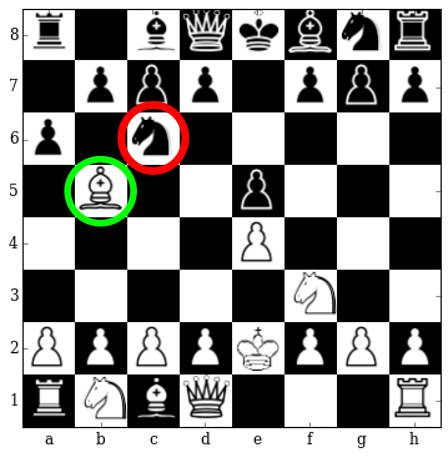
\includegraphics[scale=0.75]{img/from_to.png}
\caption{Model Overview}
\label{figure:model_overview}
\justifying
\small The green circle is the position to be predicted by the \textsc{Piece} 
selector network, while the red circle is the position to be predicted by the 
\textsc{Bishop} move selector network.
\end{figure}
A move in chess is characterized by legal movement of a friendly piece. The 
selected piece is moved onto one of the positions depending on factors like its 
ability to jump over another piece or not, whether the final position already 
has a friendly piece, whether the move doesn't cause a check etc. We divide 
this task into two simple steps--choose a piece, choose its final position. 
Given a board, we predict the next move by simply making the 
predictions in this order. While learning we consider the moves from the 
dataset as gold standard and minimize our loss functions in order to make the 
network learn certain generalizations, rules and even strategies. In 
figure~\ref{figure:model_overview}, the two different colored circles represent 
these two tasks. A formulation of this process would be:
\[P(move | board) = P(from|board)\times P(to|from, board)\]
To learn the probability function, we make use of Convolutional Neural 
Networks. Each of the different types of pieces has its own independently 
trained network, namely-- \textsc{Pawn}, \textsc{Rook}, \textsc{Knight}, 
\textsc{Bishop}, \textsc{Queen} and \textsc{King}, while the piece selector 
network is named \textsc{Piece}.\\

The network used for both piece selector and move selectors are shown below:\\
\begin{figure}[H]
\includegraphics[width=1.0\textwidth,center]{img/net1.png}
\caption{Network Architecture: ChessNet-1}
\small\centering
This network was used for piece and move predictions.
\label{figure:network1}
\end{figure}
The convolutional neural network shown in figure~\ref{figure:network1} consists 
of input layer of size $8\times 8\times 6$ (or $8\times 8\times 12$ depending 
on the choice of representation, described in 
section~\ref{section:representation12}), an output layer of size 64 which 
predicts the position of the piece to be moved. The other specifications of the 
network are:
\begin{itemize}
 \item \textbf{Convolutional Layer}-- 
 \begin{enumerate}
  \item filter size =$3\times 3$ each of depth 6
  \item number of filters=$64$
  \item padding=1
 \end{enumerate}
 \item Non-linearity-- \textbf{ReLU} $max(0,x)$
 \item \textbf{Convolutional Layer}-- 
 \begin{enumerate}
  \item filter size =$3\times 3$ each of depth 64
  \item number of filters=$96$
  \item padding=1
 \end{enumerate}
 \item Non-linearity-- \textbf{ReLU} $max(0,x)$
 \item \textbf{Convolutional Layer}-- 
 \begin{enumerate}
  \item filter size =$3\times 3$ each of depth 96
  \item number of filters=$256$
  \item padding=1
 \end{enumerate}
 \item Non-linearity-- \textbf{ReLU} $max(0,x)$
 \item \textbf{Fully connected layer}-- dimensions=1024
 \item Softmax (Loss) Layer -- \textbf{Softmax}, 
 $p_k=\frac{e^{o_k}}{\sum_i e^{o_i}}$, $o_k$ is the activation at the last 
fully connected layer in the network.
\end{itemize}

While training, the softmax layer is replaced by a softmax loss layer, output 
for the softmax loss layer is defined as follows:
\[L = - \sum_j y_j log p_j\]
where L is the loss, $y_j$ is 0 or 1 depending on the actual 
label.\label{section:lossfunc} The 
derivative of the loss function can be derived as follows:
\begin{align*}
 \frac{\partial L}{\partial o_i} &= -\sum_k y_k\frac{\partial log p_k}{\partial 
o_i} \\
&= -\sum_k y_k \frac{1}{p_k}\frac{\partial p_k}{\partial o_i}\\
&= -y_i(1-p_i) - \sum_{k\neq i} y_k \frac{1}{p_k}(-p_kp_i)\\
&= p_i\bigg(\sum_k y_k\bigg) - y_i\\
&= p_i-y_i
\end{align*}

\section{Learning the evaluation function}
\label{section:eval-func}
In addition to a piece and move predictor, we also learn an evaluation 
function. Since we want to be consistent with not injecting any domain 
knowledge for the game of chess to our models, we formulate the task of 
learning the evaluation function as regression problem with the evaluations of 
the boards inspired by TD-Learning \cite{Barto89learningand, 
sutton1988learning}. Particularly, without using any other knowledge of the 
game, we simply assign discounted reward values to the board as its evaluation. 
Starting with the final leaf nodes (after which no more gameplay is possible or 
one of the player has resigned), we assign board values to be 1 for the winning 
player's board view, -1 for the losing player's board 
view\footnote{Since we are learning from white's perspective, the player's 
board view refers to how the board would have looked to the player if he was 
playing as a white i.e. the board flipped across the horizontal as well 
flipped by color.} and 0 for both if it was a draw. This assignment is the same 
as that 
described as an optimal evaluation function for chess given the fully expanded 
game tree described in~\ref{section:solving}. But for the preceding board 
positions, we assign a discounted reward value as the valuation using a 
discounting factor represented by $\gamma$, where $0\leq \gamma \leq 1$.
\[V(b_{t_{final}}) = \begin{cases}
1 \text{ , if White has won}\\
0 \text{ , if it is a draw}\\
-1 \text{ , if Black has won}
\end{cases}\]
According to the recursive rule the discounted reward for a board at time $t$ 
into the game is:
\[V(t) = \gamma V(t+1) , \forall t<t_{final}\]
Use the following rule moving up into the game:
\[V(b_{t_{final}-i}) = \begin{cases}
		\gamma^{i} \text{ , if white won eventually}\\
                -\gamma^{i} \text{ , if black won eventually}\\
                0 \text{ , if the game was a draw}\\
               \end{cases}\]
\[V(b'_{t_{final}-i}) = \begin{cases}
		-\gamma^{i} \text{ , if white won eventually}\\
                \gamma^{i} \text{ , if black won eventually}\\
                0 \text{ , if the game was a draw}\\
               \end{cases}\]
where $b_{t_{final}-i}$ is the board (as it appears to the white player) $i$ 
steps away from the finish, while $b'_{t_{final}-i}$ is the rotated board with 
flipped colors i steps away from the finish.\\

Since the learning is done offline (in our case using game databases), we 
simulate the whole game before assigning values to each board appearing in the 
board. Now, each board position seen in the data has some evaluation that is 
based on the final outcome of the game. It is intuitive to say that a player who 
is seeing a higher valued board is more likely to win. And higher the value of 
the current board, the closer I am to winning the game and vice versa.\\

We model the task of learning such an evaluation function as regression problem 
on the network shown in figure~\ref{figure:network2}.
\begin{figure}[h]
\includegraphics[width=1.0\textwidth,center]{img/net3.png}

\caption{Network Architecture: ChessNet-2}
\small\centering
This network was used for regression to learn the evaluation function. The 
difference from the network in~\ref{figure:network1}, other than the dimensions 
of output, is the type of non-linearity used. In this network we use $tanh$, 
rather than ReLU since we need values to range from -1 to 1. We also tried 
other non-linear activation functions like leaky ReLU or a sigmoid function 
with no significant difference in results.
\label{figure:network2}
\end{figure}

The input layer size is $6\times 8\times 8$, while the output layer size is 1 
i.e. the evaluation function's value for the input board. The loss function 
optimized to train the network is the \textit{mean squared error} which is the 
basic linear regression loss function.
\[L = \frac{1}{2}(f(x)-y)^2\] where x is the value at the last fully 
connected layer in the network and f is the activation function (tanh in our 
case).
Simply the gradient looks like:
\[\frac{\partial L}{\partial x} = (f(x)-y)\frac{\partial f(x)}{\partial x}\]

The backward pass for rest of the layers works in the same way as the previous 
network.

\section{Playing}
\label{section:playing}
In this section we will look at the algorithms we use during the gameplay to 
decide which move to play depending on the outputs of our models. The first two 
algorithms do not make use of search and just make predictions based on the 
current table, while the rest mix the predictions or evaluations made by our 
model with a search based mechanism to predict the next move.

\section{Choosing a move}
The output by each of the networks for a given input board (with or without the 
augmented channels) is a probability distribution over the whole board. The 
probability distribution output by the trained \textsc{Piece} network, call it 
$P_{piece}$, is a 64-dimensional vector where each value denotes the probability 
of moving the piece at the corresponding position on the board. Similarly, the 
probability distribution output by the $i^{th}$ \textsc{Move} network, call it 
$P_{move,i}$, is a 64-dimensional vector where each value denotes the 
probability of moving a piece of type $i$ to that particular position. We use 
two or more of these probabilities to choose the complete move (initial and the 
final position) using one of the methods described below.
\subsection{Top-move method}
Simply choose the piece at position with the maximum probability in the 
\textsc{Piece} network's output. Determine its piece type and input the same 
board to the type's \textsc{Move} network. Choose the final position with the 
maximum probability.
\begin{algorithm}[H]
\begin{algorithmic}[1]
 	\State initial\_pos = argmax($P_{piece}(board)$)\;
   	\State piece\_type = getType(initial\_pos)\;
   	\State final\_pos = \funccall{argmax}($P_{move,piece\_type}(board)$)\;
   	\Return chess\_coords(initial\_pos)+chess\_coords(	final\_pos)\;
\end{algorithmic}
\caption{Top-move method}
\label{alg:topmove}
\end{algorithm}

\subsection{Top-prob method}
\label{subsection:topprob}
Rather than just determining the distribution of the moves originating from the 
most probable piece, we can also generate the full cumulative probability 
distribution for every possible from-to pair. This method is based on the 
principle that: 
\[P(move | board ) = P(piece | board )\times 
P(final\_position|piece, board)\]

\begin{algorithm}[H]
 \begin{algorithmic}[1]
 	\State piece\_dist = $P_{piece}(board)$
   	\State cumulative\_dist = \funccall{zeros}(64,64)
   	\For {$0\leq i<64$}
   		\If {$board[i/8,i\% 8]\neq 0$}
   			\State piece\_type=\funccall{getType}(i)
   			\State move\_distr = $P_{move,piece\_type}(board)$ * 
piece\_distr[i]
   			\State cumulative\_distr[i] = move\_distr
   		\EndIf
   	\EndFor
   	\State initial\_pos, final\_pos = \funccall{argmax}(cumulative\_distr)
   	\Return \funccall{chess\_coords}(initial\_pos)+\funccall{chess\_coords}	
(	final\_pos)
 \end{algorithmic}
 \caption{Top-prob method}
 \label{alg:topprob}
\end{algorithm}

\subsection{TopProb-Negamax Interleaved}
\label{subsection:interleaved}
In this method we interleave our method of evaluating moves with negamax, which 
is a kind of minmax search algorithm. We will 
describe both Negamax and our pruning method interleaved with Negamax.
The basic idea is that we will reduce the search space for the Negamax 
algorithm and also provide it with an evaluation metric for the moves or the 
boards.\\
%XXX
The Negamax algorithm is derived from Minimax algorithm. However it differs in 
the way that it utilizes the same subroutine for the Min player and the Max 
player at each step, passing on the negated score following the rule:
\[max(a,b) = -min(-a,-b)\]
\begin{algorithm}[h]
 \begin{algorithmic}[1]
 	\Procedure{Negamax}(depth)
 	\If {depth==0} 
	  \Return \funccall{evaluate}()
 	\EndIf
 	\State max = $-\infty$
 	\State \funccall {generateMoves}($\dots$)
 	\While {m = \funccall{getNextMove}()}
	  \State \funccall{makeMove}(m)
	  \State score = -\funccall{Negamax}(depth -1)
	  \State \funccall{unmakeMove}(m)
	  \If {score $>$ max}
	    \State max = score
	  \EndIf
	\EndWhile
	\Return max
    \EndProcedure
 \end{algorithmic}
 \caption{The basic Negamax algorithm for Chess}
 \label{alg:negamax}
\end{algorithm}
 The functions $makeMove$ and $unmakeMove$, as the names suggest, make the move 
on the board before calling Negamax again for the child nodes, and then un-make 
the move to search the subtrees of the siblings.

However, the function calls of our interest is the $generateMoves$ and 
$evaluate$. $generateMoves$ function uses chess logic to generate 
legal moves, which are then explored using recursion, while $evaluate$ uses the 
player's evaluation function to return the value for a leaf node.\\

For our case, we can modify the $generateMoves$ procedure to actually just 
generate a reduced number of moves available at every board position, hence 
pruning the search tree. The reduced number of moves are generated in a way 
similar to algorithm~\ref{alg:topprob}, where we generate a 
cumulative probability distribution of size $64\times 64$. The difference being 
that rather than making a move, we just explore the subtree of the generated 
move. In the same way as before, we can make use of transposition tables to 
store the values of boards already evaluation while expansion of the tree.\\

Our idea of making a narrower and deeper search of the game tree instead of a 
full width and shallow search is motivated by \citealp*{de1996perception} as 
discussed in chapter~\ref{chap:background}.\\

For $evaluate$ function call, we simply ask our network to evaluate one or a 
batch of boards. The function is better described earlier in 
the section~\ref{section:eval-func}.

\section{Training: Implementation details and Hyper parameters}
\label{section:hyperparams}
We performed all our training and testing for the piece and move prediction 
models on a deep learning library named Caffe \cite{jia2014caffe} using its 
Python API. However, we couldn't use Caffe for the 
regression training and related experiments because of convergence issues. The 
implementation for the regression training to learn the 
evaluation function was done using a Theano-based deep learning library named 
Keras \cite{keras}. The complete source code of our implementation is available 
on \url{https://github.com/ashudeep/convchess}. \\

All the experiments were run on a machine with NVIDIA GeForce GTX 760 GPU with 
Cuda v6.5.\\

Move prediction models: We experimented with different hyperparameters for the 
learning procedure and 
obtained our best models at: base learning rate  of $\alpha=0.1$ and a batch 
size of 1000. We used AdaGrad to compute the updates. The learning rate was 
kept 
constant for the first $50,000$ iterations before reducing it to 0.01. The move 
prediction networks in Caffe were trained uptil $300,000$ iterations which took 
about 2-3 days.\\

Evaluation Function learning: We used a learning rate of 0.001 and RMSprop with 
a learning rate decay of 0.9 to minimize the mean squared error. We use a batch 
size of 1024. We varied the values of $\gamma$ (described in section 
\ref{section:eval-func}) between 0.7 and 0.99 to train separate models. The 
results and analysis for each of them are described in this chapter.\\
